\documentclass[11pt,a4paper]{article}

% === Packages ===
\usepackage[utf8]{inputenc}
\usepackage[T1]{fontenc}
\usepackage{amsmath,amssymb}
\usepackage{graphicx}
\usepackage{booktabs}
\usepackage{hyperref}
\usepackage[margin=1in]{geometry}
\usepackage{xcolor}
\usepackage{enumitem}
\usepackage{natbib}
\usepackage{caption}
\usepackage{subcaption}
\usepackage{float}
\usepackage{array}
\usepackage{algorithm}
\usepackage{algpseudocode}
\usepackage{tikz}
\usetikzlibrary{shapes.geometric,arrows.meta,positioning,fit,calc,patterns}
\usepackage{multirow}
\usepackage{pgfplots}
\pgfplotsset{compat=1.18}

\newcolumntype{L}[1]{>{\raggedright\arraybackslash}p{#1}}

% === Hyperlink styling ===
\hypersetup{
  colorlinks=true,
  linkcolor=blue!70!black,
  citecolor=blue!70!black,
  urlcolor=blue!70!black
}

% === Title ===
\title{\textbf{Domain-Constrained Retrieval: Failure Prevention and\\Curation Signals for Typed Knowledge Bases}}

\author{
  Raj Navakoti \\
  \texttt{rajnavakoti@gmail.com}
}

\date{June 2026}

\begin{document}

\maketitle

% =============================================================================
% ABSTRACT
% =============================================================================
\begin{abstract}
Retrieval-augmented generation (RAG) systems typically treat knowledge bases as flat document collections, ignoring structural information about entity types, knowledge layers, and typed relationships. When deployed against typed, layered knowledge bases---where entities are categorized by type and organized into semantic layers---this structural blindness leads to silent retrieval failures: the system returns plausible but incomplete or irrelevant context, and neither the user nor the system knows what was missed. We present \textbf{Domain-Constrained Retrieval (DCR)}, a seven-stage retrieval pipeline designed for typed knowledge bases. DCR introduces intent-aware query understanding, typed graph traversal, confidence-weighted scoring, multi-layer deduplication, and---as its primary novel contribution---\textbf{gap detection}, which converts retrieval dead-ends into actionable curation signals. We evaluate DCR against two baselines (naive vector search and vanilla RAG) on a synthetic healthcare claims knowledge base containing 408 entities across 18 types and 6 layers, using 50 evaluation questions across 3 independent trials per condition. DCR significantly reduces catastrophic retrieval failures: MISSING answers drop from 12.7\% (vanilla RAG) to 4.7\% ($\chi^2$ test, $p = 0.024$). On single-layer questions where the knowledge exists, DCR achieves 1.0\% MISSING compared to 12.5\% for vanilla RAG. Stage-by-stage ablation reveals that retrieval stage contributions are density-dependent: intent classification and graph traversal add noise on dense knowledge bases (408 entities) but are hypothesized to help on bounded-context knowledge bases (50--80 entities). Gap detection fires on 82\% of questions regardless of answer quality, acting as a continuous knowledge base health probe rather than a retrieval confidence signal; preliminary evidence suggests high-severity coverage gaps may predict retrieval failure, though this requires validation at scale. We report per-question stability across trials and find that pipeline complexity inversely correlates with scoring consistency---a methodological observation with implications for RAG evaluation practice.
\end{abstract}

\noindent\textbf{Keywords:} retrieval-augmented generation, typed knowledge bases, gap detection, domain-constrained retrieval, knowledge curation, entity-relationship retrieval

\vspace{1em}

% =============================================================================
% 1. INTRODUCTION
% =============================================================================
\section{Introduction}
\label{sec:introduction}

Retrieval-augmented generation has become the dominant approach for grounding large language models in domain-specific knowledge~\citep{lewis2020rag}. The standard RAG pipeline embeds documents as vectors, retrieves the top-$k$ most similar chunks to a query, and passes them as context to a generative model. This works well when the knowledge base is a flat collection of documents with uniform structure.

Enterprise knowledge bases are rarely flat. In domains such as healthcare claims processing, financial operations, and supply chain management, knowledge is inherently \emph{typed}: systems differ from processes, APIs differ from data models, business terminology differs from technical jargon. These entities exist in typed relationships---a system implements a capability, a process triggers events, a team owns a service---and are organized into semantic layers ranging from structural definitions to behavioral workflows to organizational ownership.

When a standard RAG pipeline encounters such a knowledge base, it has no mechanism to exploit this structure. Vector similarity treats a system entity and a jargon definition identically. There is no way to traverse typed relationships to discover relevant context that is semantically distant but structurally connected. Most critically, there is no way to detect what the retrieval \emph{missed}: if a question requires knowledge about a process that coordinates two systems, and the knowledge base documents the systems but not the coordination, the pipeline returns the system entities and produces a plausible-sounding but incomplete answer. The failure is silent.

We present \textbf{Domain-Constrained Retrieval (DCR)}, a seven-stage retrieval pipeline designed for typed, layered knowledge bases. DCR addresses three problems that standard RAG ignores:

\begin{enumerate}[nosep]
  \item \textbf{Type-aware retrieval.} DCR classifies query intent to determine which entity types and knowledge layers are most relevant, uses typed graph traversal to follow relationship edges, and applies layer-priority boosting during fusion.
  \item \textbf{Failure prevention.} Confidence-weighted scoring adjusts entity relevance based on content density, preventing the pipeline from returning shallow or poorly-documented entities when richer alternatives exist.
  \item \textbf{Gap detection.} DCR's novel contribution: converting retrieval dead-ends---orphan entities with no relationships, ambiguous type assignments, thin coverage areas---into structured signals that tell knowledge curators what to improve.
\end{enumerate}

We evaluate DCR on a synthetic healthcare claims knowledge base containing 408 entities across 18 types and 6 knowledge layers. Our experimental design uses 50 evaluation questions, 9 retrieval conditions (3 baselines + 6 ablation), and 3 independent trials per condition (1,350 total evaluations). We report three main findings:

\begin{enumerate}[nosep]
  \item DCR significantly reduces catastrophic retrieval failures (MISSING answers: 4.7\% vs.\ 12.7\% for vanilla RAG, $p = 0.024$), though overall answer quality improvement is not statistically significant ($p = 0.059$).
  \item The MISSING reduction concentrates in single-layer questions (12.5\% $\to$ 1.0\%), while cross-cutting questions remain at $\sim$83\% INCOMPLETE regardless of retrieval method---exposing knowledge base content gaps that retrieval cannot fix.
  \item Stage contributions are density-dependent: intent classification and graph traversal reduce accuracy on this dense knowledge base, while confidence scoring is the load-bearing stage whose removal doubles MISSING on cross-cutting questions.
\end{enumerate}

The remainder of this paper is organized as follows. Section~\ref{sec:related} surveys related work. Section~\ref{sec:pipeline} describes the DCR pipeline architecture. Section~\ref{sec:setup} details the experimental setup. Sections~\ref{sec:results} and~\ref{sec:analysis} present results and analysis. Section~\ref{sec:discussion} discusses implications, and Section~\ref{sec:conclusion} concludes.

% =============================================================================
% 2. RELATED WORK
% =============================================================================
\section{Related Work}
\label{sec:related}

\subsection{Retrieval-Augmented Generation}

RAG systems augment language model generation with retrieved context to improve factual grounding~\citep{lewis2020rag}. Early systems use dense retrieval with a single vector index. More recent work introduces hybrid retrieval combining dense and sparse methods~\citep{chen2024bge}, multi-step retrieval with query decomposition~\citep{press2023selfask}, and self-reflective retrieval where the model decides whether to retrieve~\citep{asai2024selfrag}. These advances improve retrieval quality on unstructured document collections but do not exploit typed entity structure.

\subsection{Knowledge Graph-Enhanced Retrieval}

Graph-based retrieval augments vector search with structured knowledge. GraphRAG~\citep{edge2024graphrag} builds community summaries from document graphs for global queries. GRAG~\citep{hu2024grag} integrates subgraph retrieval with text generation. These approaches construct graphs from unstructured text via entity extraction. DCR differs fundamentally: it operates on \emph{pre-existing} typed knowledge bases where entity types, relationships, and layers are defined by a domain meta-model, not extracted from text. This enables type-aware query understanding and typed edge traversal that post-hoc extraction cannot support.

\subsection{Retrieval Evaluation}

LLM-as-judge evaluation~\citep{zheng2023judging} is widely used but introduces scoring variance. \citet{shankar2024validates} show that single-judge setups have low inter-rater reliability. ConsJudge~\citep{liu2025consjudge} trains judges via DPO on consistent vs.\ inconsistent judgment pairs to improve reliability. Our evaluation uses a single LLM judge with multi-trial averaging to characterize variance, and we report inter-rater reliability (Cohen's $\kappa = 0.634$) as a methodological contribution.

\subsection{Enterprise and Domain-Specific RAG}

Enterprise RAG applications face challenges distinct from open-domain QA: structured domain knowledge, specialized terminology, regulatory constraints, and the need to audit retrieval provenance. Recent work addresses RAG for regulatory compliance~\citep{sarmah2024hybridrag}, medical knowledge retrieval, and code-specific contexts. However, these approaches typically adapt general RAG to domain-specific \emph{content} while retaining flat retrieval architectures. DCR differs by adapting to domain-specific \emph{structure}---exploiting entity types, knowledge layers, and typed relationships that are inherent to enterprise knowledge organization.

\subsection{Schema-Aware Retrieval}

A parallel line of work exploits typed schemas at query time. NL2SQL systems~\citep{rajkumar2022nl2sql} use database schemas to constrain query generation; enterprise search engines use faceted metadata (document type, department, date) to filter results. DCR extends this principle to knowledge base retrieval: entity types and relationship schemas constrain intent classification, graph traversal, and gap detection. Unlike NL2SQL, DCR operates on semi-structured entity descriptions rather than relational tables, and unlike faceted search, it uses schema structure for \emph{retrieval scoring}, not just filtering.

\subsection{Gap Detection in Information Retrieval}

Knowledge base completeness assessment is studied in the context of knowledge graph completion~\citep{bordes2013transe} and open-domain QA~\citep{rajpurkar2018squad}. However, these approaches focus on \emph{what the model cannot answer} rather than \emph{what the knowledge base is missing}. DCR's gap detection operates at the retrieval layer, identifying structural deficiencies (orphan entities, ambiguous types, thin coverage) independently of answer quality. This positions gap detection as a curation signal rather than an evaluation metric.

% =============================================================================
% 3. THE DCR PIPELINE
% =============================================================================
\section{The DCR Pipeline}
\label{sec:pipeline}

DCR operates on typed knowledge bases structured according to a domain meta-model. The meta-model defines entity types (e.g., \textit{system}, \textit{process}, \textit{team}, \textit{API}), knowledge layers (e.g., \textit{structural}, \textit{behavioral}, \textit{organizational}), and typed relationships between entities. Each entity has a type, a layer assignment, a confidence score reflecting curation quality, and a set of typed relationships to other entities.

Figure~\ref{fig:ontology} illustrates the meta-model structure. The pipeline processes a query through seven stages. Figure~\ref{fig:pipeline} shows the architecture.

\begin{figure*}[t]
\centering
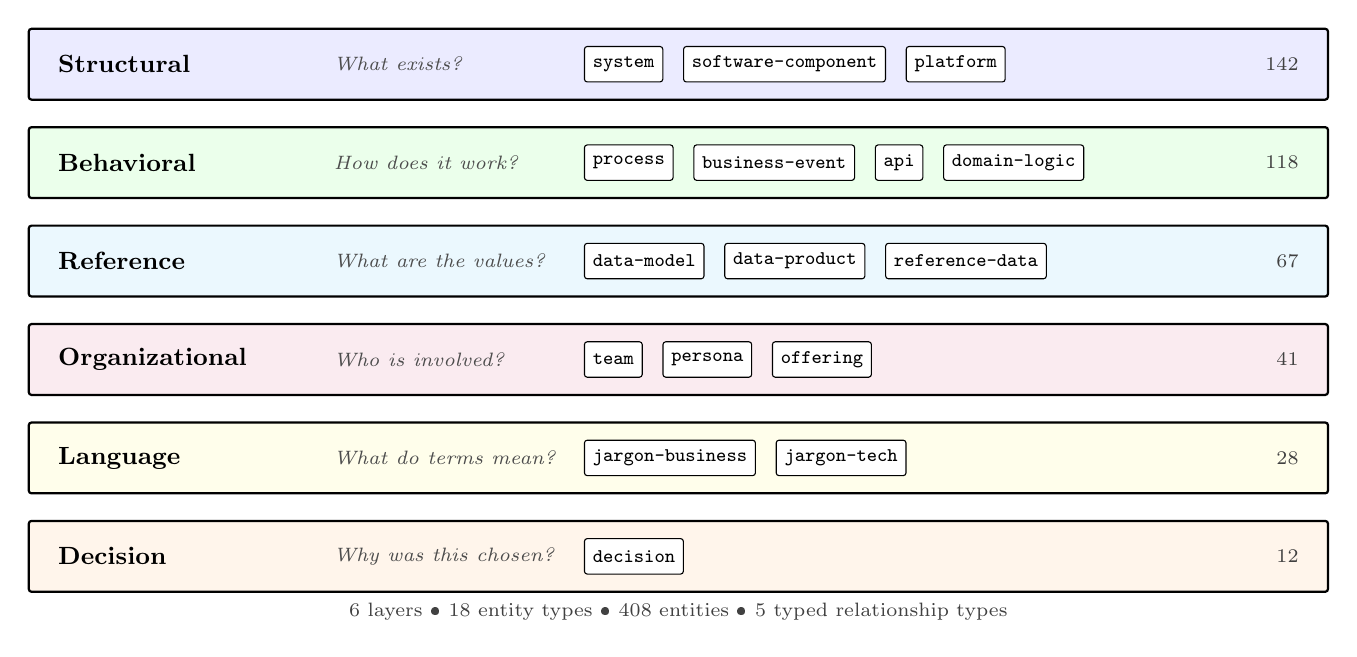
\begin{tikzpicture}[
  layer/.style={draw, thick, minimum width=16.5cm, minimum height=0.9cm, rounded corners=1pt},
  typebox/.style={draw, fill=white, font=\scriptsize\ttfamily, minimum height=0.45cm, rounded corners=1pt, inner sep=3pt},
  lbl/.style={font=\small\bfseries, anchor=west},
  qlbl/.style={font=\scriptsize\itshape, text=gray!60!black, anchor=west},
  cnt/.style={font=\scriptsize, text=gray!50!black, anchor=east},
]

\def\rowsep{1.25}
\def\typestart{-1.2}
\def\typegap{0.25cm}

% --- Structural ---
\node[layer, fill=blue!8] at (0,0) {};
\node[lbl] at (-8.0,0) {Structural};
\node[qlbl] at (-4.5,0) {What exists?};
\node[typebox, anchor=west] (s1) at (\typestart,0) {system};
\node[typebox, right=\typegap of s1] (s2) {software-component};
\node[typebox, right=\typegap of s2] (s3) {platform};
\node[cnt] at (8.0,0) {142};

% --- Behavioral ---
\node[layer, fill=green!8] at (0,-\rowsep) {};
\node[lbl] at (-8.0,-\rowsep) {Behavioral};
\node[qlbl] at (-4.5,-\rowsep) {How does it work?};
\node[typebox, anchor=west] (b1) at (\typestart,-\rowsep) {process};
\node[typebox, right=\typegap of b1] (b2) {business-event};
\node[typebox, right=\typegap of b2] (b3) {api};
\node[typebox, right=\typegap of b3] (b4) {domain-logic};
\node[cnt] at (8.0,-\rowsep) {118};

% --- Reference ---
\node[layer, fill=cyan!8] at (0,-2*\rowsep) {};
\node[lbl] at (-8.0,-2*\rowsep) {Reference};
\node[qlbl] at (-4.5,-2*\rowsep) {What are the values?};
\node[typebox, anchor=west] (r1) at (\typestart,-2*\rowsep) {data-model};
\node[typebox, right=\typegap of r1] (r2) {data-product};
\node[typebox, right=\typegap of r2] (r3) {reference-data};
\node[cnt] at (8.0,-2*\rowsep) {67};

% --- Organizational ---
\node[layer, fill=purple!8] at (0,-3*\rowsep) {};
\node[lbl] at (-8.0,-3*\rowsep) {Organizational};
\node[qlbl] at (-4.5,-3*\rowsep) {Who is involved?};
\node[typebox, anchor=west] (o1) at (\typestart,-3*\rowsep) {team};
\node[typebox, right=\typegap of o1] (o2) {persona};
\node[typebox, right=\typegap of o2] (o3) {offering};
\node[cnt] at (8.0,-3*\rowsep) {41};

% --- Language ---
\node[layer, fill=yellow!8] at (0,-4*\rowsep) {};
\node[lbl] at (-8.0,-4*\rowsep) {Language};
\node[qlbl] at (-4.5,-4*\rowsep) {What do terms mean?};
\node[typebox, anchor=west] (l1) at (\typestart,-4*\rowsep) {jargon-business};
\node[typebox, right=\typegap of l1] (l2) {jargon-tech};
\node[cnt] at (8.0,-4*\rowsep) {28};

% --- Decision ---
\node[layer, fill=orange!8] at (0,-5*\rowsep) {};
\node[lbl] at (-8.0,-5*\rowsep) {Decision};
\node[qlbl] at (-4.5,-5*\rowsep) {Why was this chosen?};
\node[typebox, anchor=west] (d1) at (\typestart,-5*\rowsep) {decision};
\node[cnt] at (8.0,-5*\rowsep) {12};

% --- Summary ---
\node[font=\scriptsize, text=gray!50!black] at (0,-5*\rowsep - 0.7) {6 layers \textbullet{} 18 entity types \textbullet{} 408 entities \textbullet{} 5 typed relationship types};

\end{tikzpicture}
\caption{The typed, layered knowledge base meta-model. Each row groups entity types that answer a category of domain question. Entities carry typed relationships across layers (e.g., \texttt{depends\_on}, \texttt{owned\_by}). DCR exploits this structure for intent classification, graph traversal, and gap detection.}
\label{fig:ontology}
\end{figure*}

\begin{figure}[t]
\centering
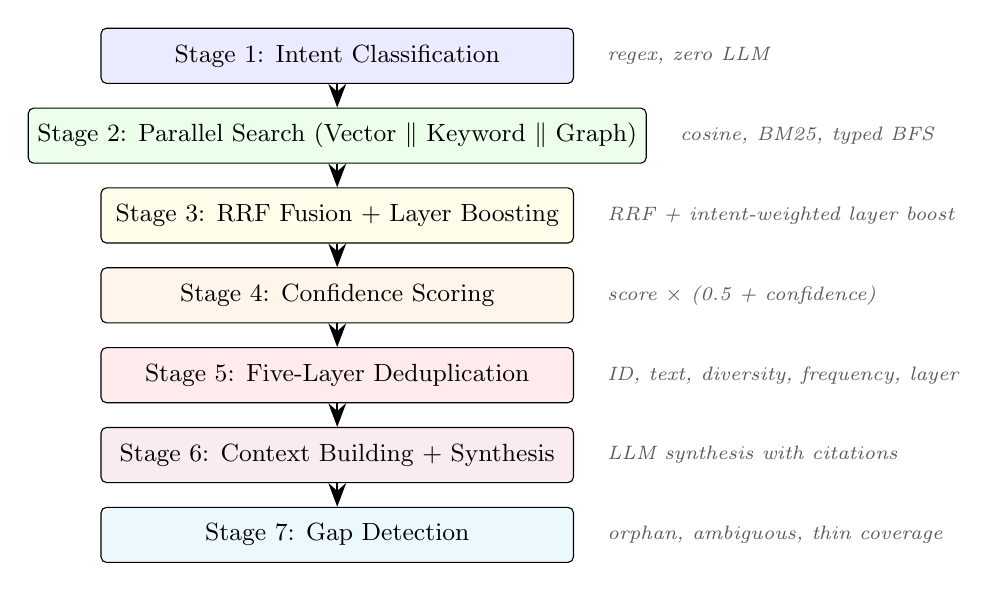
\begin{tikzpicture}[
  stage/.style={draw, rounded corners=2pt, minimum width=6cm, minimum height=0.7cm, font=\small, align=center},
  arrow/.style={-{Stealth[length=3mm]}, thick},
  note/.style={font=\scriptsize\itshape, text=gray!70!black}
]
\node[stage, fill=blue!8] (s1) {Stage 1: Intent Classification};
\node[stage, fill=green!8, below=0.3cm of s1] (s2) {Stage 2: Parallel Search (Vector $\parallel$ Keyword $\parallel$ Graph)};
\node[stage, fill=yellow!8, below=0.3cm of s2] (s3) {Stage 3: RRF Fusion + Layer Boosting};
\node[stage, fill=orange!8, below=0.3cm of s3] (s4) {Stage 4: Confidence Scoring};
\node[stage, fill=red!8, below=0.3cm of s4] (s5) {Stage 5: Five-Layer Deduplication};
\node[stage, fill=purple!8, below=0.3cm of s5] (s6) {Stage 6: Context Building + Synthesis};
\node[stage, fill=cyan!8, below=0.3cm of s6] (s7) {Stage 7: Gap Detection};

\draw[arrow] (s1) -- (s2);
\draw[arrow] (s2) -- (s3);
\draw[arrow] (s3) -- (s4);
\draw[arrow] (s4) -- (s5);
\draw[arrow] (s5) -- (s6);
\draw[arrow] (s6) -- (s7);

\node[note, right=0.3cm of s1] {regex, zero LLM};
\node[note, right=0.3cm of s2] {cosine, BM25, typed BFS};
\node[note, right=0.3cm of s3] {RRF + intent-weighted layer boost};
\node[note, right=0.3cm of s4] {score $\times$ (0.5 + confidence)};
\node[note, right=0.3cm of s5] {ID, text, diversity, frequency, layer};
\node[note, right=0.3cm of s6] {LLM synthesis with citations};
\node[note, right=0.3cm of s7] {orphan, ambiguous, thin coverage};
\end{tikzpicture}
\caption{The seven-stage DCR pipeline. Stages 1--5 handle retrieval; Stage 6 synthesizes an answer; Stage 7 detects knowledge base gaps. All stages except Stage 6 are deterministic.}
\label{fig:pipeline}
\end{figure}

\subsection{Stage 1: Intent Classification}

Intent classification determines which entity types and knowledge layers are most relevant to the query. DCR uses a zero-LLM approach: regex pattern matching against the query text to assign weights to eight fixed, hand-designed intent categories (process, ownership, entity, relationship, temporal, diagnostic, listing, comparison). These categories are not learned; they were derived from manual analysis of 200+ enterprise support questions across three domains during prior work on the Demand-Driven Context methodology~\citep{navakoti2026ddc}. Each intent maps to a weight vector over entity types and knowledge layers. For example, a process query increases weights for \textit{process}, \textit{business-event}, and \textit{workflow} entity types and boosts the \textit{behavioral} knowledge layer.

\subsection{Stage 2: Parallel Search}

Three search strategies run concurrently:

\begin{itemize}[nosep]
  \item \textbf{Vector search.} The query is embedded and compared against entity embeddings using cosine similarity. Returns the top-$K$ candidates, where $K$ is automatically scaled to 20\% of entity count (81 entities for this knowledge base). This threshold balances recall (surfacing relevant entities across types) against context window limits; we acknowledge this default was not ablated and note it as a limitation.
  \item \textbf{Keyword search.} BM25-style scoring against entity names and body text.
  \item \textbf{Graph search.} Breadth-first traversal from the top vector results, following typed relationship edges. Edge types are filtered based on query intent: a process query follows \texttt{triggers}, \texttt{depends\_on}, and \texttt{implements} edges but not \texttt{owned\_by}. Maximum depth is 3 hops.
\end{itemize}

\subsection{Stage 3: RRF Fusion with Layer Boosting}

Reciprocal Rank Fusion~\citep{cormack2009rrf} merges the three candidate lists. The fused score is blended with the original cosine similarity: $s = 0.7 \times s_{\text{RRF}} + 0.3 \times s_{\text{cosine}}$. Layer priority boosting then adjusts scores based on the intent-derived layer weights from Stage~1.

\subsection{Stage 4: Confidence Scoring}

Each entity carries a confidence score (0.0--1.0) reflecting its curation quality---how complete its description is, how many relationships are documented, and how many source documents support it. Confidence scoring adjusts the retrieval score: $s' = s \times (0.5 + c)$, where $c$ is the entity's confidence. The 0.5 floor ensures that even minimally documented entities retain half their retrieval score rather than being zeroed out; a pure multiplicative model ($s' = s \times c$) would eliminate newly created entities before curation could validate them. Additional boosts account for relationship density ($\log(1 + \text{edge\_count})$) and source document count.

\subsection{Stage 5: Five-Layer Deduplication}

Deduplication applies five sequential filters: (1) exact entity ID dedup, (2) text similarity dedup (cosine $> 0.85$ on body text), (3) type diversity enforcement (limits entities per type based on intent), (4) inverse frequency weighting (deprioritizes ubiquitous entities), and (5) layer diversity enforcement (ensures representation across knowledge layers).

\subsection{Stage 6: Context Building and Synthesis}

Retrieved entities are assembled into a structured context window. An LLM synthesizes an answer with entity-level citations. The LLM also self-scores the answer as ANSWERABLE, PARTIAL, or NOT\_ANSWERABLE, which we map to CLEAN, INCOMPLETE, and MISSING respectively.

\subsection{Stage 7: Gap Detection}

Gap detection examines the retrieval trace to identify three types of knowledge base deficiencies:

\begin{itemize}[nosep]
  \item \textbf{Orphan entities.} Entities retrieved with high relevance but no typed relationships to other retrieved entities---indicating missing relationship documentation.
  \item \textbf{Ambiguous entities.} Pairs of retrieved entities with high name or content similarity but different types---indicating potential duplicates or unclear type boundaries.
  \item \textbf{Thin coverage.} Retrieved entity count meets the top-$K$ threshold but content density is low across the result set---indicating that the knowledge base lacks depth in this area.
\end{itemize}

Gap detection is downstream of retrieval and independent of answer quality. Its output is a structured list of gap signals, each with a type, severity, and description. These signals are designed for knowledge base curators, not end users.

% =============================================================================
% 4. EXPERIMENTAL SETUP
% =============================================================================
\section{Experimental Setup}
\label{sec:setup}

\subsection{Knowledge Base}

We use a synthetic healthcare claims processing domain: Clearview Health Plans, a fictional regional health insurer. The knowledge base contains 408 entities across 18 types and 6 knowledge layers (Table~\ref{tab:kb-stats}).

The knowledge base was constructed in three stages. First, 148 synthetic source documents were generated describing the domain's systems, processes, APIs, data models, teams, and terminology. Second, an automated extraction pipeline (Claude Sonnet with a typed meta-model schema) processed each document to identify entities, assign types and layers, extract relationships, and generate confidence scores based on description completeness, relationship density, and source document coverage. Third, extracted entities underwent manual curation review: deduplication, relationship validation, and quality assessment. The pipeline and source documents are included in the repository.

\begin{table}[h]
\centering
\caption{Knowledge base composition by layer.}
\label{tab:kb-stats}
\begin{tabular}{@{}lcc@{}}
\toprule
Layer & Entity Types & Entity Count \\
\midrule
Structural & 3 & 142 \\
Behavioral & 4 & 118 \\
Reference & 3 & 67 \\
Organizational & 3 & 41 \\
Language & 2 & 28 \\
Decision & 1 & 12 \\
\midrule
\textbf{Total} & \textbf{18} & \textbf{408} \\
\bottomrule
\end{tabular}
\end{table}

\subsection{Evaluation Questions}

We generated 50 evaluation questions from seed context using an LLM, then deduplicated using a dual threshold: Jaccard similarity $> 0.55$ on question tokens and entity overlap $> 0.7$ on extracted entity references. Questions span two categories: 18 cross-cutting questions requiring synthesis across multiple entity types and layers, and 32 single-layer questions addressable from entities within a single knowledge layer.

\subsection{Conditions}

We evaluate 9 retrieval conditions: 3 baselines and 6 ablation variants.

\paragraph{Baselines.}
\begin{itemize}[nosep]
  \item \textbf{Naive vector.} Cosine similarity only. No keyword search, no graph traversal, no fusion.
  \item \textbf{Vanilla RAG.} Vector search plus keyword search with simple score averaging. No typed traversal, no confidence scoring, no dedup beyond ID matching.
  \item \textbf{DCR.} Full seven-stage pipeline.
\end{itemize}

\paragraph{Ablation.} Each variant removes one stage from the full DCR pipeline:
\begin{itemize}[nosep]
  \item \textbf{full\_dcr}: control (identical to DCR baseline, run separately to measure scoring variance).
  \item \textbf{no\_intent}: Stage 1 removed; flat layer weights.
  \item \textbf{no\_graph}: Stage 2 graph traversal removed; vector + keyword only.
  \item \textbf{no\_layer\_boost}: Stage 3 layer priority boosting removed from fusion.
  \item \textbf{no\_confidence}: Stage 4 confidence scoring removed.
  \item \textbf{no\_dedup}: Stage 5 multi-layer dedup replaced with simple ID dedup.
\end{itemize}

\subsection{Scoring}

Each retrieved context is passed to Claude Sonnet\footnote{Model ID: \texttt{claude-sonnet-4-6} (API identifier \texttt{claude-4-sonnet-20250514}), Anthropic's Claude Sonnet 4 release (May 2025). Accessed via Anthropic API.} for synthesis and self-scoring in a single LLM call. The model generates an answer with entity citations and, on the final line, self-scores as ANSWERABLE, PARTIAL, or NOT\_ANSWERABLE. We map these to:

\begin{itemize}[nosep]
  \item \textbf{CLEAN}: the knowledge base fully addresses the question.
  \item \textbf{INCOMPLETE}: the knowledge base partially addresses the question but key information is missing.
  \item \textbf{MISSING}: the knowledge base does not contain enough information to answer.
\end{itemize}

The same model is used for both synthesis and scoring. While this introduces a potential self-enhancement bias~\citep{zheng2023judging}, we mitigate it in three ways: (1) multi-trial averaging reduces single-run bias, (2) the inter-rater reliability check (Section~\ref{sec:judge}) re-scores answers \emph{without} retrieval context, removing the synthesis framing, and (3) we report relative comparisons across conditions rather than absolute quality claims---any systematic bias affects all conditions equally.

Each condition is run 3 independent times (different LLM scoring runs on identical retrieval results) to characterize scoring variance. Total evaluations: 50 questions $\times$ 9 conditions $\times$ 3 trials = 1,350.

\subsection{Judge Consistency}
\label{sec:judge}

We assessed inter-rater reliability by re-scoring 15 stratified (question, answer) pairs (5 CLEAN, 8 INCOMPLETE, 2 MISSING) through the same LLM judge twice. Self-consistency was 100\% (15/15). Agreement with original scoring was 80\% (12/15). Cohen's $\kappa = 0.634$ (substantial agreement). We note that $n = 15$ is below the typical minimum for reliability studies; the kappa provides a directional but not statistically powered reliability estimate. All 3 disagreements were one-directional promotions of borderline cases (MISSING $\to$ INCOMPLETE or INCOMPLETE $\to$ CLEAN), indicating conservative original scoring.

\textbf{Cross-model validation.} To address same-model self-bias, we scored 30 (question, answer) pairs using GPT-4o as an independent judge: 15 from DCR and 15 from vanilla RAG, each stratified as 5 CLEAN, 7 INCOMPLETE, 3 MISSING. Cross-model agreement with Claude's original scoring was 80.0\% (24/30), identical to Claude's self-agreement rate. All 6 disagreements were promotions (3 per condition), affecting both conditions equally. GPT-4o confirms the conservative scoring pattern without distorting the relative comparison between retrieval pipelines.

% =============================================================================
% 5. RESULTS
% =============================================================================
\section{Results}
\label{sec:results}

\subsection{Baseline Comparison}

Table~\ref{tab:baselines} shows the baseline comparison. DCR achieves the lowest MISSING rate (4.7\% $\pm$ 2.3) with modest CLEAN improvement over baselines. Note that LLM scoring variance introduces a $\sim$4pp noise floor: the ablation's full\_dcr condition (Table~\ref{tab:ablation}), an identical pipeline scored in a separate trial batch, reports 38.0\% CLEAN vs.\ 34.0\% here. Section~\ref{sec:stability} discusses this variance in detail.

\begin{table}[h]
\centering
\caption{Baseline comparison (mean $\pm$ SD across 3 trials, $n = 50$ questions).}
\label{tab:baselines}
\begin{tabular}{@{}lccc@{}}
\toprule
Condition & CLEAN (\%) & INCOMPLETE (\%) & MISSING (\%) \\
\midrule
Naive Vector & $30.0 \pm 3.5$ & $60.7 \pm 2.3$ & $9.3 \pm 3.1$ \\
Vanilla RAG & $30.0 \pm 0.0$ & $57.3 \pm 2.3$ & $12.7 \pm 2.3$ \\
DCR (ours) & $34.0 \pm 2.0$ & $61.3 \pm 4.2$ & $\mathbf{4.7 \pm 2.3}$ \\
\bottomrule
\end{tabular}
\end{table}

The MISSING reduction from vanilla RAG to DCR is statistically significant. We constructed a $2 \times 2$ contingency table (MISSING vs.\ non-MISSING $\times$ DCR vs.\ vanilla RAG, pooling all 150 observations per condition): DCR produced 7 MISSING and 143 non-MISSING; vanilla RAG produced 19 MISSING and 131 non-MISSING. Chi-square test: $\chi^2 = 5.10$, $df = 1$, $p = 0.024$.

For overall score comparison, we encoded DDC classes as ordinal values (CLEAN $= 3$, INCOMPLETE $= 2$, MISSING $= 1$) and applied the Mann-Whitney U test across 150 observations per condition: $U = 10307.5$, $p = 0.059$, not significant at $\alpha = 0.05$.

\subsection{Ablation Study}

Table~\ref{tab:ablation} shows the effect of removing individual pipeline stages.

\begin{table}[h]
\centering
\caption{Ablation study---stage contribution (mean $\pm$ SD across 3 trials). The full\_dcr row is an identical pipeline to DCR in Table~\ref{tab:baselines}, scored in a separate trial batch; the 4pp CLEAN difference reflects LLM scoring variance.}
\label{tab:ablation}
\begin{tabular}{@{}lcccc@{}}
\toprule
Condition & CLEAN (\%) & INCOMPLETE (\%) & MISSING (\%) & $\Delta$ CLEAN \\
\midrule
full\_dcr & $38.0 \pm 6.0$ & $56.7 \pm 6.4$ & $5.3 \pm 4.2$ & --- \\
no\_intent & $44.7 \pm 4.2$ & $49.3 \pm 4.2$ & $6.0 \pm 2.0$ & $+6.7$ \\
no\_graph & $40.7 \pm 1.2$ & $53.3 \pm 3.1$ & $6.0 \pm 2.0$ & $+2.7$ \\
no\_layer\_boost & $37.3 \pm 3.1$ & $59.3 \pm 4.2$ & $3.3 \pm 1.2$ & $-0.7$ \\
no\_confidence & $35.3 \pm 4.2$ & $56.0 \pm 5.3$ & $8.7 \pm 1.2$ & $-2.7$ \\
no\_dedup & $39.3 \pm 1.2$ & $56.0 \pm 2.0$ & $4.7 \pm 1.2$ & $+1.3$ \\
\bottomrule
\end{tabular}
\end{table}

Two findings stand out. First, removing intent classification \emph{increases} CLEAN by 6.7 percentage points, and removing graph traversal increases it by 2.7pp. This counterintuitive result is discussed in Section~\ref{sec:density}. Second, removing confidence scoring decreases CLEAN by 2.7pp \emph{and} increases MISSING to 8.7\%---the highest among all ablation conditions. Confidence scoring is the one stage whose removal degrades both precision and failure prevention.

\subsection{Scoring Variance}

The baseline DCR condition and the ablation full\_dcr condition run identical pipeline code. Their CLEAN scores differ by 4 percentage points (34.0\% vs.\ 38.0\%), with full\_dcr exhibiting higher variance (SD $= 6.0$ vs.\ $2.0$). This gap---pure LLM scoring variance on identical retrieval---establishes the noise floor for interpreting all results.

\subsection{Per-Question Stability}
\label{sec:stability}

Table~\ref{tab:stability} reports the percentage of questions that received the same DDC class across all 3 trials.

\begin{table}[h]
\centering
\caption{Per-question stability (same DDC class across 3 trials).}
\label{tab:stability}
\begin{tabular}{@{}lcc@{}}
\toprule
Condition & Stable Questions & Stability (\%) \\
\midrule
no\_layer\_boost & 44/50 & 88 \\
vanilla\_rag & 42/50 & 84 \\
dcr & 41/50 & 82 \\
no\_dedup & 41/50 & 82 \\
no\_graph & 41/50 & 82 \\
no\_intent & 39/50 & 78 \\
naive\_vector & 37/50 & 74 \\
no\_confidence & 35/50 & 70 \\
full\_dcr & 34/50 & 68 \\
\bottomrule
\end{tabular}
\end{table}

Figure~\ref{fig:stability} visualizes the stability data. Pipeline complexity inversely correlates with stability: simpler conditions (vanilla RAG, no\_layer\_boost) are more stable than complex ones (full DCR). This suggests that more pipeline stages introduce more variance in the context passed to the LLM judge, even when the retrieval is deterministic.

\begin{figure}[t]
\centering
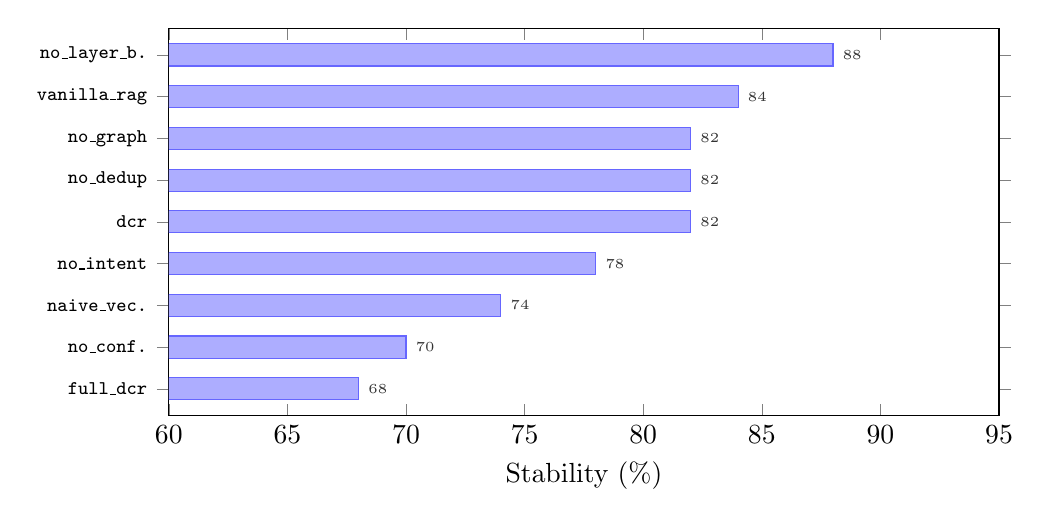
\begin{tikzpicture}
\begin{axis}[
    xbar,
    width=\columnwidth,
    height=6.5cm,
    bar width=8pt,
    xlabel={Stability (\%)},
    xmin=60, xmax=95,
    ytick={1,2,3,4,5,6,7,8,9},
    yticklabels={\texttt{full\_dcr},\texttt{no\_conf.},\texttt{naive\_vec.},\texttt{no\_intent},\texttt{dcr},\texttt{no\_dedup},\texttt{no\_graph},\texttt{vanilla\_rag},\texttt{no\_layer\_b.}},
    y tick label style={font=\scriptsize},
    nodes near coords,
    nodes near coords style={font=\tiny, anchor=west},
    every axis plot/.append style={fill opacity=0.8},
    enlarge y limits=0.08,
]
\addplot[fill=blue!40, draw=blue!60] coordinates {
  (68, 1)
  (70, 2)
  (74, 3)
  (78, 4)
  (82, 5)
  (82, 6)
  (82, 7)
  (84, 8)
  (88, 9)
};
\end{axis}
\end{tikzpicture}
\caption{Per-question stability (percentage of questions with identical DDC class across all 3 trials). Simpler pipelines achieve higher consistency; the full pipeline is least stable at 68\%.}
\label{fig:stability}
\end{figure}

% =============================================================================
% 6. ANALYSIS
% =============================================================================
\section{Analysis}
\label{sec:analysis}

\subsection{Question Difficulty Stratification}
\label{sec:stratification}

We stratified questions into two categories: 18 cross-cutting questions requiring synthesis across entity types and layers, and 32 single-layer questions addressable within a single knowledge layer. Table~\ref{tab:stratified} shows the stratified baseline results.

\begin{table}[h]
\centering
\caption{Stratified baseline results by question type.}
\label{tab:stratified}
\begin{tabular}{@{}llccc@{}}
\toprule
Group & Condition & CLEAN (\%) & INC (\%) & MISS (\%) \\
\midrule
\multirow{3}{*}{Cross-cutting ($n=18$)} & Naive Vector & 3.7 & 83.3 & 13.0 \\
 & Vanilla RAG & 1.9 & 85.2 & 13.0 \\
 & DCR & 5.6 & 83.3 & 11.1 \\
\midrule
\multirow{3}{*}{Single-layer ($n=32$)} & Naive Vector & 44.8 & 47.9 & 7.3 \\
 & Vanilla RAG & 45.8 & 41.7 & 12.5 \\
 & DCR & 50.0 & 49.0 & \textbf{1.0} \\
\bottomrule
\end{tabular}
\end{table}

Figure~\ref{fig:stratified} visualizes the stratified MISSING rates. The MISSING reduction concentrates overwhelmingly in single-layer questions: from 12.5\% (vanilla RAG) to 1.0\% (DCR), an 11.5 percentage-point drop.

\begin{figure}[t]
\centering
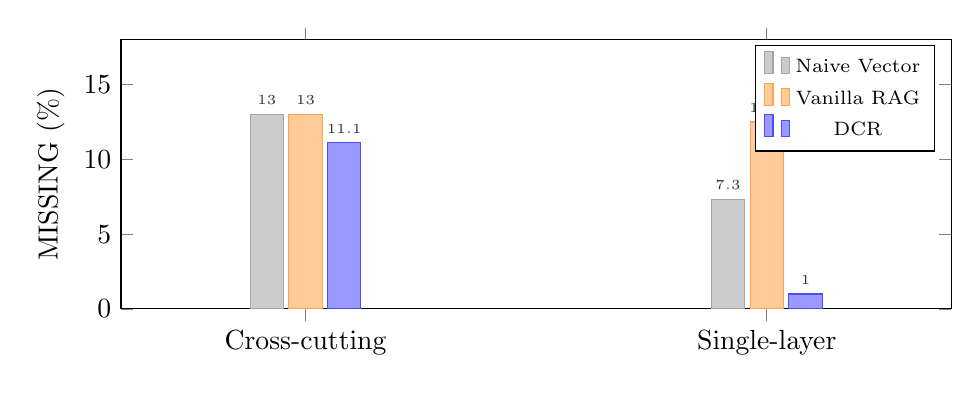
\begin{tikzpicture}
\begin{axis}[
    ybar,
    width=\columnwidth,
    height=5cm,
    bar width=12pt,
    ylabel={MISSING (\%)},
    symbolic x coords={Cross-cutting, Single-layer},
    xtick=data,
    ymin=0, ymax=18,
    legend style={at={(0.98,0.98)}, anchor=north east, font=\scriptsize, legend columns=1},
    nodes near coords,
    nodes near coords style={font=\tiny},
    every axis plot/.append style={fill opacity=0.8},
    enlarge x limits=0.4,
]
\addplot[fill=gray!50, draw=gray!70] coordinates {(Cross-cutting, 13.0) (Single-layer, 7.3)};
\addplot[fill=orange!50, draw=orange!70] coordinates {(Cross-cutting, 13.0) (Single-layer, 12.5)};
\addplot[fill=blue!50, draw=blue!70] coordinates {(Cross-cutting, 11.1) (Single-layer, 1.0)};
\legend{Naive Vector, Vanilla RAG, DCR}
\end{axis}
\end{tikzpicture}
\caption{MISSING rates stratified by question type. DCR's failure reduction concentrates in single-layer questions (12.5\% $\to$ 1.0\%), while cross-cutting questions remain at $\sim$13\% MISSING regardless of method---a knowledge base content ceiling, not a retrieval limitation.}
\label{fig:stratified}
\end{figure} Cross-cutting questions show only a 1.9pp reduction (13.0\% $\to$ 11.1\%). This separates two distinct phenomena:

\begin{itemize}[nosep]
  \item \textbf{Retrieval failure} (which DCR fixes): on single-layer questions where the answer exists in the knowledge base, DCR nearly eliminates the case where the pipeline fails to retrieve it.
  \item \textbf{Knowledge base incompleteness} (which DCR diagnoses but cannot fix): cross-cutting questions require integrated process documentation that the knowledge base lacks. The $\sim$83\% INCOMPLETE rate is a content ceiling, not a retrieval limitation.
\end{itemize}

\subsection{Confidence Scoring Across Strata}

Stratified ablation on cross-cutting questions reveals that removing confidence scoring doubles MISSING from 7.4\% to 16.7\%---the largest single-stage effect in the entire experiment. Confidence scoring is content-density-aware rather than type-aware: it adjusts entity relevance based on how well-documented the entity is, not what type it belongs to. This makes it effective regardless of knowledge base size, and particularly valuable on hard questions where retrieved entities tend to be thin.

\subsection{Gap Detection}
\label{sec:gaps}

Gap detection fires on 82\% of questions (41 of 50), producing 184 gap signals across 3 trials. Table~\ref{tab:gaps} shows the gap type distribution. Figure~\ref{fig:gaps} illustrates the three gap types with concrete examples from the experiment.

\begin{table}[h]
\centering
\caption{Gap detection results across 3 DCR trials.}
\label{tab:gaps}
\begin{tabular}{@{}lccc@{}}
\toprule
Gap Type & Count & Severity & Description \\
\midrule
Orphan entity & 90 & low & No typed relationships \\
Ambiguous entity & 87 & medium & Name/content overlap across types \\
Thin coverage & 7 & high & Content density insufficient \\
\midrule
\textbf{Total} & \textbf{184} & & \\
\bottomrule
\end{tabular}
\end{table}

\begin{figure}[t]
\centering
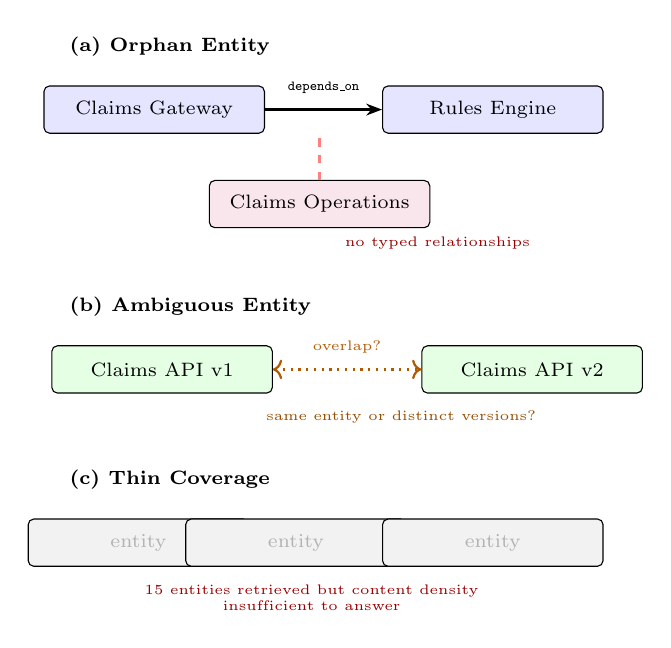
\begin{tikzpicture}[
  entity/.style={draw, rounded corners=2pt, minimum width=2.8cm, minimum height=0.6cm, font=\scriptsize, align=center},
  gap/.style={draw, dashed, rounded corners=2pt, minimum width=3cm, minimum height=0.6cm, font=\scriptsize, align=center, fill=red!5},
  edge/.style={-{Stealth[length=2mm]}, thick},
  noedge/.style={thick, dashed, red!50},
  label/.style={font=\scriptsize\bfseries, anchor=west},
]

% Orphan entity example
\node[label] at (-3.5, 0.5) {(a) Orphan Entity};
\node[entity, fill=blue!10] (e1) at (-2.3, -0.3) {Claims Gateway};
\node[entity, fill=blue!10] (e2) at (2.0, -0.3) {Rules Engine};
\node[entity, fill=purple!10] (e3) at (-0.2, -1.5) {Claims Operations};
\draw[edge] (e1) -- node[above, font=\tiny, yshift=2pt] {\texttt{depends\_on}} (e2);
\draw[noedge] (e3) -- (-0.2, -0.6);
\node[font=\tiny, text=red!60!black, anchor=west] at (0.0, -2.0) {no typed relationships};

% Ambiguous entity example
\node[label] at (-3.5, -2.8) {(b) Ambiguous Entity};
\node[entity, fill=green!10] (a1) at (-2.2, -3.6) {Claims API v1};
\node[entity, fill=green!10] (a2) at (2.5, -3.6) {Claims API v2};
\draw[thick, dotted, orange!70!black, <->] (a1) -- node[above, font=\tiny, yshift=2pt] {overlap?} (a2);
\node[font=\tiny, text=orange!60!black, anchor=west] at (-1.0, -4.2) {same entity or distinct versions?};

% Thin coverage example
\node[label] at (-3.5, -5.0) {(c) Thin Coverage};
\node[entity, fill=gray!10] (c1) at (-2.5, -5.8) {\color{gray!60}entity};
\node[entity, fill=gray!10] (c2) at (-0.5, -5.8) {\color{gray!60}entity};
\node[font=\scriptsize, text=gray!50] at (1.0, -5.8) {\dots};
\node[entity, fill=gray!10] (c3) at (2.0, -5.8) {\color{gray!60}entity};
\node[font=\tiny, text=red!60!black, align=center] at (-0.3, -6.5) {15 entities retrieved but content density\\insufficient to answer};

\end{tikzpicture}
\caption{The three gap detection types with examples from the experiment. (a)~Orphan entities have high retrieval relevance but no typed relationships to other results. (b)~Ambiguous entities share names or content across different types. (c)~Thin coverage: the entity count meets the threshold but content lacks depth. Thin coverage gaps (c) correlate with MISSING outcomes (7/7).}
\label{fig:gaps}
\end{figure}

The 9 questions (18\%) where gap detection does not fire are exclusively CLEAN or INCOMPLETE---no MISSING question escapes detection. These are single-entity definitional questions where the retrieved entities have well-documented relationships and sufficient depth.

A counterintuitive finding: gap count does \emph{not} correlate with MISSING scores. CLEAN answers average 1.39 gaps per question, while MISSING answers average 1.29. This means gap detection is not measuring retrieval failure---it is measuring knowledge base structural health. Orphan entities and ambiguous types surface regardless of whether the current query succeeds.

However, \textbf{thin coverage gaps do predict retrieval failure}: all 7 thin-coverage events in the dataset co-occurred with MISSING outcomes. While $n = 7$ is too small for statistical claims, this perfect correlation suggests high-severity coverage gaps as a potential predictor of retrieval failure. We note this should be validated on larger question sets.

Gap detection is downstream of intent classification: the \texttt{no\_intent} ablation condition detects 126 gaps compared to 184--185 for conditions with intent enabled. Without intent classification, the pipeline lacks the type expectations needed to identify orphan entities or ambiguous type assignments. This is expected behavior---a design dependency, not a deficiency.

\subsection{INCOMPLETE Characterization}

INCOMPLETE answers constitute 50--65\% of results across all conditions---the largest category. To characterize this mass, we qualitatively examined 10 randomly sampled INCOMPLETE answers from DCR. This characterization is based on qualitative inspection and should not be interpreted as a quantitative finding; no second reviewer independently assessed these cases.

All 10 share the same pattern: correct entity retrieval (15 hops per question), reasonable synthesis with entity-level citations, and explicit self-identification of what specific detail is missing. Examples include: ``800K members across three states'' with the gap being that the specific state names are not documented; a full claims processing flow missing only the final payment issuance steps; a correct definition of Coordination of Benefits missing operational exception handling.

No INCOMPLETE answer was near-MISSING. The INCOMPLETE plateau represents a \textbf{knowledge base content ceiling}: the pipeline retrieves the right entities, but those entities lack operational depth. This is precisely the signal that gap detection is designed to surface, and it reinforces DCR's role as a curation tool: it tells you not just what it found, but what you should document next.

% =============================================================================
% 7. DISCUSSION
% =============================================================================
\section{Discussion}
\label{sec:discussion}

\subsection{Density Dependence of Typed Retrieval Stages}
\label{sec:density}

The ablation study reveals a counterintuitive result: removing intent classification and graph traversal \emph{improves} CLEAN scores on this 408-entity knowledge base. This does not mean typed retrieval is harmful. It means typed stages are density-dependent.

On a dense knowledge base where entities of every type are well-represented, intent-based filtering can push relevant entities down the ranking by suppressing types that fall outside the predicted intent. For example, a process query might deprioritize \textit{system} entities that are, in fact, essential to answering the question. Graph traversal compounds this by expanding the result set along typed edges that may lead away from the most relevant entities.

We hypothesize that typed retrieval stages earn their contribution on bounded-context knowledge bases containing 50--80 entities, where disambiguation between similar entities matters and the graph is sparse enough for typed traversal to add signal rather than noise. Testing this hypothesis requires experiments on partitioned knowledge bases and is left to future work.

This distinction---between the value of a \emph{typed ontology} (entity types, layers, relationships, curated descriptions) and the value of \emph{typed retrieval stages} (intent classification, layer boosting, graph traversal)---is important. The typed ontology makes \emph{every} retrieval method better: even naive vector search achieves 30\% CLEAN on this well-structured knowledge base. The typed retrieval stages are an additional layer of pipeline complexity whose benefit depends on knowledge base density.

\subsection{Gap Detection as Curation Signal}

Gap detection's 82\% trigger rate and its independence from answer quality position it as a continuous knowledge base health probe rather than a retrieval confidence signal. Every query surfaces structural information about the knowledge base: orphan entities needing relationship documentation, ambiguous types needing clarification, and thin coverage areas needing content investment.

The thin-coverage correlation with MISSING (7/7) suggests a hierarchy of gap severity: low-severity gaps (orphans, ambiguities) are pervasive and represent ongoing curation work, while high-severity gaps (thin coverage) indicate areas where the knowledge base cannot support reliable retrieval. This hierarchy has practical implications for knowledge base maintenance: curators can prioritize thin-coverage gaps for immediate attention while treating orphan and ambiguity gaps as background improvement work.

\subsection{Evaluation Methodology}

Our multi-trial design with per-question stability analysis reveals that pipeline complexity inversely correlates with scoring consistency. Full DCR achieves 68\% stability compared to 84\% for vanilla RAG and 88\% for the simplest ablation condition. This suggests that more complex retrieval produces more varied context, which in turn produces more varied LLM scoring.

This observation has implications for RAG evaluation practice: single-trial evaluations of complex pipelines may not be reliable, and evaluation frameworks should report stability alongside accuracy. The 4-percentage-point gap between baseline DCR and ablation full\_dcr---identical pipelines scored in different trial batches---illustrates the magnitude of this variance.

\subsection{Limitations}

\begin{itemize}[nosep]
  \item \textbf{Single knowledge base.} All experiments use one synthetic domain. Generalization to other domains, knowledge base sizes, and entity type distributions is not established.
  \item \textbf{Synthetic data.} The knowledge base was generated and curated, not extracted from a production enterprise. Production knowledge bases may have different quality distributions.
  \item \textbf{LLM judge with self-scoring.} The same model (Claude Sonnet) generates and scores answers, introducing potential self-enhancement bias~\citep{zheng2023judging}. Our cross-model check (GPT-4o, $n = 30$) shows 80\% agreement with identical promotion patterns across conditions, suggesting the bias does not distort relative comparisons. However, absolute DDC class rates may differ under human evaluation.
  \item \textbf{No $K$ sensitivity analysis.} The top-$K$ retrieval threshold is auto-scaled to 20\% of entity count. This default was not ablated; different $K$ values may affect both baseline and DCR results.
  \item \textbf{Small question set.} 50 questions provide adequate statistical power for the MISSING comparison but limit analysis of per-question-type effects. The thin-coverage finding ($n = 7$) requires validation at scale.
  \item \textbf{LLM-generated questions.} The 50 evaluation questions were generated by an LLM from seed context rather than drawn from real user queries. This may bias the question type distribution toward patterns the model finds syntactically natural, underrepresenting the kinds of ad hoc or poorly phrased questions that arise in production enterprise settings.
  \item \textbf{Density hypothesis untested.} The claim that typed stages help on smaller knowledge bases is a hypothesis motivated by the ablation results, not an empirical finding in this paper.
\end{itemize}

% =============================================================================
% 8. CONCLUSION
% =============================================================================
\section{Conclusion}
\label{sec:conclusion}

We presented Domain-Constrained Retrieval, a seven-stage pipeline for typed, layered knowledge bases. DCR significantly reduces catastrophic retrieval failures ($p = 0.024$) and converts every query into a knowledge base health probe via gap detection. The MISSING reduction concentrates in single-layer questions (12.5\% $\to$ 1.0\%), while cross-cutting incompleteness exposes genuine knowledge base content gaps that no retrieval method can fix.

Stage-by-stage ablation reveals that contributions are density-dependent: confidence scoring is the load-bearing stage, while intent classification and graph traversal add noise on dense knowledge bases. This characterizes a retrieval design space rather than a pipeline failure---typed stages are hypothesized to help on bounded-context knowledge bases where disambiguation matters.

Gap detection, DCR's novel contribution, fires on 82\% of questions regardless of answer quality. It is a curation signal, not a retrieval confidence metric: it tells knowledge base curators what to document next, not whether the current answer is reliable. The thin-coverage gap type predicts retrieval failure with a perfect (7/7) but small-sample correlation.

Future work includes validating the density hypothesis by partitioning the knowledge base into bounded contexts of 50, 100, and 200 entities and re-running the same 50-question evaluation at each scale---if typed stages improve CLEAN on smaller partitions, it confirms that pipeline contributions are density-dependent rather than architecture-dependent. We also plan to scale the evaluation to 200+ questions with deterministic scoring rubrics and human-calibrated labels, and to validate gap detection's predictive power (particularly the thin-coverage $\to$ MISSING correlation) on larger datasets. We release the pipeline implementation, evaluation data, and synthetic knowledge base to support reproducibility.\footnote{\url{https://github.com/ea-toolkit/dcr-paper}}

% =============================================================================
% REFERENCES
% =============================================================================
\bibliographystyle{plainnat}

\begin{thebibliography}{99}

\bibitem[Asai et~al.(2024)]{asai2024selfrag}
A.~Asai, Z.~Wu, Y.~Wang, A.~Sil, and H.~Hajishirzi.
\newblock Self-{RAG}: Learning to retrieve, generate, and critique through self-reflection.
\newblock In \emph{ICLR}, 2024.

\bibitem[Bordes et~al.(2013)]{bordes2013transe}
A.~Bordes, N.~Usunier, A.~Garcia-Duran, J.~Weston, and O.~Yakhnenko.
\newblock Translating embeddings for modeling multi-relational data.
\newblock In \emph{NeurIPS}, 2013.

\bibitem[Chen et~al.(2024)]{chen2024bge}
J.~Chen, S.~Xiao, P.~Zhang, K.~Luo, D.~Lian, and Z.~Liu.
\newblock {BGE} {M3}-Embedding: Multi-lingual, multi-functionality, multi-granularity text embeddings through self-knowledge distillation.
\newblock \emph{arXiv preprint arXiv:2402.03216}, 2024.

\bibitem[Cormack et~al.(2009)]{cormack2009rrf}
G.~V.~Cormack, C.~L.~A.~Clarke, and S.~B{\"u}ttcher.
\newblock Reciprocal rank fusion outperforms {Condorcet} and individual rank learning methods.
\newblock In \emph{SIGIR}, 2009.

\bibitem[Edge et~al.(2024)]{edge2024graphrag}
D.~Edge, H.~Trinh, N.~Cheng, J.~Bradley, A.~Chao, A.~Mody, S.~Truitt, and J.~Larson.
\newblock From local to global: A graph {RAG} approach to query-focused summarization.
\newblock \emph{arXiv preprint arXiv:2404.16130}, 2024.

\bibitem[Hu et~al.(2024)]{hu2024grag}
Z.~Hu, Z.~Xu, G.~Qi, and K.~Wang.
\newblock {GRAG}: Graph retrieval-augmented generation.
\newblock \emph{arXiv preprint arXiv:2405.16506}, 2024.

\bibitem[Navakoti and Navakoti(2026)]{navakoti2026ddc}
R.~Navakoti and S.~Navakoti.
\newblock Demand-driven context: A methodology for building enterprise knowledge bases through agent failure.
\newblock \emph{arXiv preprint arXiv:2603.14057}, 2026.

\bibitem[Sarmah et~al.(2024)]{sarmah2024hybridrag}
B.~Sarmah, B.~Hall, R.~Rao, S.~Patel, S.~Pasupuleti, and M.~Kulkarni.
\newblock {HybridRAG}: Integrating knowledge graphs and vector retrieval augmented generation for efficient information extraction.
\newblock \emph{arXiv preprint arXiv:2408.04948}, 2024.

\bibitem[Lewis et~al.(2020)]{lewis2020rag}
P.~Lewis, E.~Perez, A.~Piktus, F.~Petroni, V.~Karpukhin, N.~Goyal, H.~K{\"u}ttler, M.~Lewis, W.-t.~Yih, T.~Rockt{\"a}schel, S.~Riedel, and D.~Kiela.
\newblock Retrieval-augmented generation for knowledge-intensive {NLP} tasks.
\newblock In \emph{NeurIPS}, 2020.

\bibitem[Liu et~al.(2025)]{liu2025consjudge}
S.~Liu, J.~Li, Y.~Cao, and others.
\newblock Judge as a judge: Improving the evaluation of retrieval-augmented generation through the judge-consistency of large language models.
\newblock In \emph{Findings of ACL}, 2025.

\bibitem[Press et~al.(2023)]{press2023selfask}
O.~Press, M.~Zhang, S.~Min, L.~Schmidt, N.~A.~Smith, and M.~Lewis.
\newblock Measuring and narrowing the compositionality gap in language models.
\newblock In \emph{Findings of EMNLP}, 2023.

\bibitem[Rajkumar et~al.(2022)]{rajkumar2022nl2sql}
N.~Rajkumar, R.~Li, and D.~Baber.
\newblock Evaluating the text-to-{SQL} capabilities of large language models.
\newblock \emph{arXiv preprint arXiv:2204.00498}, 2022.

\bibitem[Rajpurkar et~al.(2018)]{rajpurkar2018squad}
P.~Rajpurkar, R.~Jia, and P.~Liang.
\newblock Know what you don't know: Unanswerable questions for {SQuAD}.
\newblock In \emph{ACL}, 2018.

\bibitem[Shankar et~al.(2024)]{shankar2024validates}
S.~Shankar, J.~Zamfirescu-Pereira, B.~Hartmann, A.~Parameswaran, and I.~Arawjo.
\newblock Who validates the validators? {A}ligning {LLM}-assisted evaluation of {LLM} outputs with human preferences.
\newblock In \emph{UIST}, 2024.

\bibitem[Zheng et~al.(2023)]{zheng2023judging}
L.~Zheng, W.-L.~Chiang, Y.~Sheng, S.~Zhuang, Z.~Wu, Y.~Zhuang, Z.~Lin, Z.~Li, D.~Li, E.~P.~Xing, H.~Zhang, J.~E.~Gonzalez, and I.~Stoica.
\newblock Judging {LLM}-as-a-judge with {MT-Bench} and {Chatbot Arena}.
\newblock In \emph{NeurIPS}, 2023.

\end{thebibliography}

\end{document}
